% -- Anfang Präambel
\documentclass[german,  % Standardmäßig deutsche Eigenarten, englisch -> english
parskip=full,  % Absätze durch Leerzeile trennen
%bibliography=totoc,  % Literatur im Inhaltsverzeichnis (ist unüblich)
%draft,  % TODO: Entwurfsmodus -> entfernen für endgültige Version
]{scrartcl}
\usepackage[utf8]{inputenc}  % Kodierung der Datei
\usepackage[T1]{fontenc}  % Vollen Umfang der Schriftzeichen
\usepackage[ngerman]{babel}  % Sprache auf Deutsch (neue Rechtschreibung)

% Mathematik und Größen
\usepackage{amsmath}
\usepackage[locale=DE,  % deutsche Eigenarten, englisch -> US
separate-uncertainty,  % Unsicherheiten seperat angeben (mit ±)
]{siunitx}
\usepackage{physics}  % Erstellung von Gleichungen vereinfachen
\usepackage{yfonts}  % Frakturschrift für Real- und Imaginärteil komplexer Größen

\usepackage{graphicx}  % Bilder einbinden \includegraphics{Pfad/zur/Datei(ohne Dateiendung)}

% Gestaltung
%\usepackage{microtype}  % Mikrotypographie (kann man am Ende verwenden)
\usepackage{booktabs}  % schönere Tabellen
%\usepackage[toc]{multitoc}  % mehrspaltiges Inhaltsverzeichnis
\usepackage{csquotes}  % Anführungszeichen mit \enquote
\usepackage{caption}  % Anpassung der Bildunterschriften, Tabellenüberschriften
\usepackage{subcaption}  % Unterabbildungen, Untertabellen, …
\usepackage{enumitem}  % Listen anpassen
\setlist{itemsep=-10pt}  % Abstände zwischen Listenpunkten verringern

% Manipulation des Seitenstils
\usepackage{scrpage2}
% Kopf-/Fußzeilen setzen
\pagestyle{scrheadings}  % Stil für die Seite setzen
\clearscrheadings  % Stil zurücksetzen, um ihn neu zu definieren
\automark{section}  % Abschnittsnamen als Seitenbeschriftung verwenden
\ofoot{\pagemark}  % Seitenzahl außen in Fußzeile
\ihead{\headmark}  % Seitenbeschriftung mittig in Kopfzeile
\setheadsepline{.5pt}  % Kopzeile durch Linie abtrennen

\usepackage[hidelinks]{hyperref}  % Links und weitere PDF-Features

% TODO: Titel und Autor, … festlegen
\newcommand*{\titel}{Holographie}
\newcommand*{\autor}{Tom Drechsler, Konstantin Schmid}
\newcommand*{\abk}{HO}
\newcommand*{\betreuer}{Karla Roszeitis}
\newcommand*{\messung}{14.11.2019}
\newcommand*{\ort}{<Ort>}

\hypersetup{pdfauthor={\autor}, pdftitle={\titel}}  % PDF-Metadaten setzen

% automatischen Titel konfigurieren
\titlehead{Fortgeschrittenen-Praktikum \abk \hfill TU Dresden}
\subject{Versuchsprotokoll}
\title{\titel}
\author{\autor}
\date{\begin{tabular}{ll}
Protokoll: & \today\\
Messung: & \messung\\
Ort: & \ort\\
Betreuer: & \betreuer\end{tabular}}

% -- Ende Präambel

\begin{document}
\begin{titlepage}
\maketitle  % Titel setzen
\tableofcontents  % Inhaltsverzeichnis
\end{titlepage}

% Text Anfang
\section{Versuchsziel und Überblick}
Der Versuch hat das Ziel, sich mit Komponenten und Arbeitstechniken in einem Laserlabor vertraut zu machen. 
\newline Zuerst wird ein Michelson-Interferometer aufgebaut und Stabilität sowie Kohärenzlänge werden untersucht. Danach wird die Holographie-Anordnung für Weißlicht-Reflexionshologramme aufgebaut und schließlich das Hologramm aufgezeichnet, entwickelt und untersucht. Als Vorkenntnisse werden Elektrodynamik, Fourieranalyse und das Grundprinzip des Lasers benötigt, welche im Folgenden nochmal zusammengefasst sind.

\section{Theoretische Grundlagen}
\subsection{Das Grundprinzip der Holographie}
Klassische Fotografie hat den Nachteil, dass bloß die Intensitätsverteilung reproduziert werden kann und so die Phaseninformation der einfallenden Wellen, wie beschrieben durch Gleichung (\ref{ÜberlagerungWelle}), verloren geht.
\begin{align}
\label{ÜberlagerungWelle} \vec{E}=\sum_{i}\vec{a}_i \cos(\vec{k} \vec{r} - \omega t - \varphi_i)
\end{align}
In der Holographie wird das Lichtfeld des Objektes mit einer Referenzwelle überlagert und bei der Rekonstruktion des Lichtmusters wird das Hologramm wieder mit dieser Referenzwelle beleuchtet, sodass die rekonstruierte Welle in Phase und Amplitude der Originalwelle entspricht.

\subsection{Mathematische Grundlagen und Definitionen}
\subsubsection{Intensität elektromagnetischer Wellen}
Die tatsächliche Intensität elektromagnetischer Strahlung ist ein Maß für die Energie pro Fläche und Zeitintervall. Im Allgemeinen wird die tatsächliche Intensität $I_{\mathrm{t}}$ mit Hilfe des Poynting-Vektors $\vec{S}$ über die Gleichung (\ref{Poynting}) bestimmt.
\begin{align}
\label{Poynting} I_{\mathrm{t}}=| \langle \vec{S} \rangle |
\end{align}
Dies vereinfacht sich in linearen Medien zu (\ref{LineareMedien})
\begin{align}
\label{LineareMedien} I_{\mathrm{t}}(t)= \varepsilon_0 c n \vec{E}^2 \stackrel{n=1}{=} \varepsilon_0 c \vec{E}(t)^2
\end{align}
Durch zeitliche Mittelung ergibt sich der finale Ausdruck für die Intensität:
\begin{align}
\label{Intensität} I = \langle I_{\mathrm{t}} \rangle = \lim\limits_{T \rightarrow \infty} \frac{1}{T} \int_{- \frac{T}{2}}^{\frac{T}{2}} I_{\mathrm{t}}(t) \ \mathrm{d}t = \varepsilon_0 c  \langle \vec{E}^2 \rangle
\end{align}
Im allgemeinen Fall wird tatsächlich der gesamte Vektor \(\vec{E}(\vec{r},t)\) benötigt. Wir betrachten im folgenden ausschließlich den Spezialfall für \textbf{linear polarisiertes} Licht. Hier oszilliert der Feldstärkevektor \(\vec{E}(\vec{r},t)\) in einer festen Ebene. Da man das Koordinatensystem beliebig wählen kann, ist es keine Einschränkung wenn man 
\[\vec{E}(\vec{r},t) = E(\vec{r},t)\vec{e}_x\]
d.h. \(\vec{E}\parallel\vec{e}_x\) legt. Dann ist aber \(\vec{E}(\vec{r},t)^2 = E(\vec{r},t)^2\), weshalb es ausreichend ist, mit \textbf{skalaren} Größen zu rechnen. Wir lassen daher ab sofort den Vektorpfeil weg. Außerdem ist für viele Rechnungen sehr praktisch, elektromagnetische Wellen durch die komplexe Exponentialfunktion zu beschreiben. Für die ebene Welle mit harmonischer Zeit- und Ortsabhängigkeit
\[E(\vec{r},t) = E_0 \cos (\vec{k}\vec{r} - \Omega t)\]
führt man das komplexe elektrische Feld \(\hat{E}\) ein:
\[\hat{E}(\vec{r},t) = E_0 \mathrm{e}^{\mathrm{i}(\vec{k}\vec{r} - \Omega t)} = E_0 \left[\cos (\vec{k}\vec{r} - \Omega t) + \mathrm{i}\sin (\vec{k}\vec{r} - \Omega t)\right]\]
Aus diesem ergibt sich das beobachtbare reelle elektrische Feld \(E\) durch Bildung des Realteils:
\[E(\vec{r},t) = \textfrak{Re} \ \hat{E}(\vec{r},t) = \frac{1}{2}\left(\hat{E}(\vec{r},t) + \hat{E}^{*}(\vec{r},t)\right)\]
wobei \(^{*}\) die komplexe Konjugation bedeutet. Mithilfe des komplexen Feldes \(\hat{E}\) kann das Betragsquadrat des elektrischen Feldstärkevektors umformuliert werden und (\ref{Intensität}) wird zu:
\begin{align}
\label{Intensität2} I = \frac{1}{2} \varepsilon_0 c \langle \hat{E} \hat{E^*} \rangle
\end{align}

\subsubsection{Die Fourierdarstellung}
Das Fourierspektrum des reellen elektrischen Feldes ist definiert als:
\begin{align}
\label{Fourierspektrum} H(\omega) = \int_{- \infty}^{\infty}  E(t) e^{\mathrm{i}\omega t}  \ \mathrm{d}t, \omega \geq 0
\end{align}
Da allerdings für kontinuierliche Strahlung die Gesamtenergie divergiert, verwendet man stattdessen eine mittlere Leistung, wozu man einen zeitlichen Ausschnitt $E_T$ von $E(t)$ benötigt. Das dementsprechende Fourierspektrum $H_T(\omega)$ kann man analog über (\ref{Fourierspektrum}) ermitteln. Als Grenzwert findet man dann die spektrale Dichte S($\omega$):
\begin{align}
\label{SpektraleDichte} S(\omega)= \frac{1}{\pi} \lim\limits_{T \rightarrow \infty} \frac{|H_T(\omega)|^2}{T}
\end{align}
Mit dieser ist es möglich die mittlere Intensität als Integral über $S(\omega)$ auszudrücken:
\begin{align}
\label{Intensität3} I=\varepsilon_0 c \int_{0}^{\infty} S(\omega) \ \mathrm{d} \omega
\end{align}

\subsubsection{Die Interferenz von Wellen}
Als Ansatz betrachten wir zwei sich überlagernde ebene harmonische Wellen, gegeben durch (\ref{Welle})
\begin{align}
\label{Welle} \hat{E_i}=a_i e^{\mathrm{i}(\vec{k}_i \vec{r} - \omega t - \varphi_i)}, i=1,2
\end{align}
Im Folgenden bezeichnet $\hat{E}_{tot}$ die Superposition der beiden einzelnen Amplituden.
Die totale mittlere Intensität der beiden Wellen ist dann:
\begin{align}
\label{Intensität4} I_{\mathrm{tot}}(\vec{r})=\frac{1}{2} \varepsilon_0 c \langle \hat{E}_{\mathrm{tot}} \hat{E}_{\mathrm{tot}}^* \rangle = 
I_1 + I_2 + 2\sqrt{I_1 I_2}\cdot \cos(\phi(\vec{r})) \,\,\text{mit}\,\, \phi(\vec{r}) = (\vec{k}_1 - \vec{k}_2) \vec{r} - (\varphi_1 - \varphi_2)
\end{align}

\subsection{Kohärenz und Kontrastfunktion}
\subsubsection{Ebene Wellen und reale Wellenzüge}
Alle bisherigen Überlegungen wurden mit ebenen Wellen durchgeführt. Diese bilden das denkbar einfachste Modell und erfüllen auch die Maxwell'schen Gleichungen. Sie haben allerdings den Nachteil, dass sie der Realität nur bedingt nahe kommen: Da die ebenen Wellen mathematisch durch Sinus- und Cosinusfunktionen oder die komplexe Exponentialfunktion beschrieben werden, sind sie zwangsläufig sowohl zeitlich als auch örtlich unendlich weit ausgedehnt. Jede reale Lichtquelle sendet aber stets nur Wellenzüge von endlicher Länge aus. Das hat aber eine recht unangenehme Konsequenz: Betrachten wir beispielsweise einen Wellenzug, die während des Zeitintervalls \(\left[-\frac{T}{2},\frac{T}{2}\right]\) durch eine ebene Welle beschrieben werden kann und davor und danach verschwindet:
\[\hat{E}(\vec{r},t) = E_0 \mathrm{e}^{\mathrm{i}(\vec{k}\vec{r} - \Omega t)} \cdot\left[\Theta\left(t+\frac{T}{2}\right) - \Theta\left(t-\frac{T}{2}\right)\right]\]
mit der Heaviside-Funktion \(\Theta\). Die Fouriertransformierte des Realteils von \(\hat{E}\) im Zeitbereich liefert dann das Frequenzspektrum von \(E\):
\begin{align*}
H(\omega) = \int_{-\infty}^{\infty} \mathrm{e}^{\mathrm{i}\omega t}\textfrak{Re} \ \hat{E}(\vec{r},t) \ \mathrm{d} t = \hdots = E_0 \left\lbrace   \frac{\sin\left[(\omega - \Omega)\frac{T}{2}\right]}{\omega - \Omega} \cdot \mathrm{e}^{\mathrm{i}\vec{k}\vec{r}} +  \frac{\sin\left[(\omega + \Omega)\frac{T}{2}\right]}{\omega + \Omega} \cdot \mathrm{e}^{-\mathrm{i}\vec{k}\vec{r}}\right\rbrace
\end{align*}
Für die spezielle Wahl \(\vec{r} = \vec{\mathrm{o}}\) ist das Frequenzspektrum in der folgenden Abbildung dargestellt:
\begin{figure}[h!]\centering
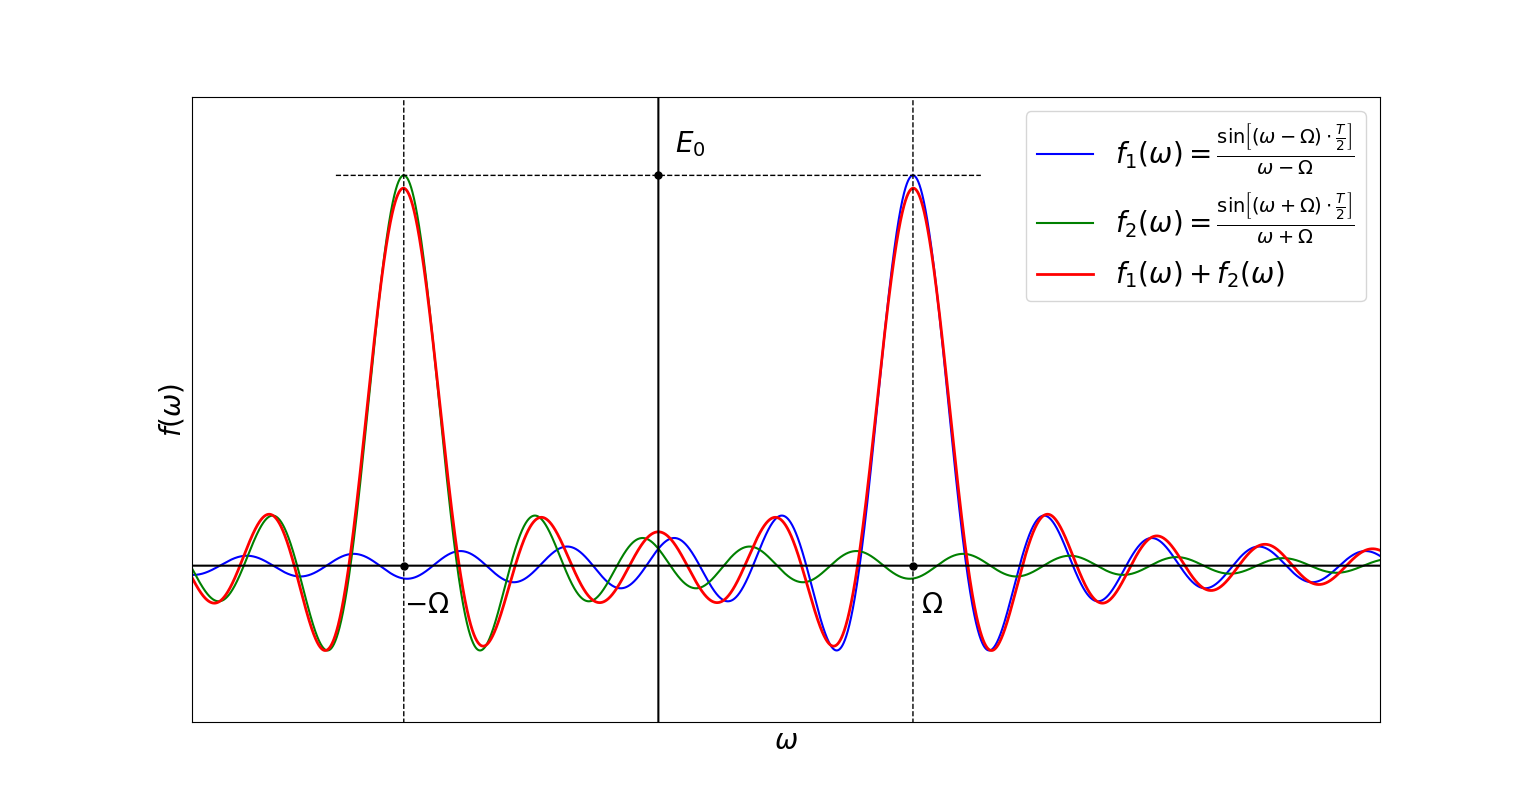
\includegraphics[scale=0.4]{Frequenzspektrum.png}
\label{Frequenzspqktrum}
\caption{Frequenzspektrum \(H(\omega)\) bei \(\vec{r} = \vec{\mathrm{o}}\), in willkürlichen Einheiten}
\end{figure}

Für Orte \(\vec{r}\neq \vec{\mathrm{o}}\) kommt es lediglich zu einer örtlichen Oszillation, die wir im folgenden nicht weiter betrachten. Auffällig ist, dass das Spektrum \(H(\omega)\) für große \(\omega\) im wesentlichen vom ersten Summanden bestimmt wird, weil die Funktion \(\frac{\sin(x)}{x}\) ein sehr ausgeprägtes Maximum hat und dann rasch abfällt. Da \(H\) ohnehin nur für positive \(\Omega\) benötigt wird, kann man in sehr guter Näherung schreiben:
\begin{align}
H(\omega) \approx E_0 \mathrm{e}^{\mathrm{i}\vec{k}\vec{r}}\cdot \frac{\sin\left[(\omega - \Omega)\frac{T}{2}\right]}{\omega - \Omega}  
\end{align}
Für die spektrale Energiedichte ergibt sich - abgesehen von numerischen Faktoren durch Ensemblemittelung - der gleiche funktionale Zusammenhang:
\begin{align}
S(\omega) \sim \frac{\sin^2\left[(\omega - \Omega)\frac{T}{2}\right]}{(\omega - \Omega)^2}  
\end{align}
Man kann sich anhand von \ref{Frequenzspqktrum} leicht klar machen, dass \(S\) einen scharfen Peak bei \(\omega=\Omega\) hat. Die nächsten beiden Nullstellen sind dann offenbar die Nullstellen der Sinusfunktion im Zähler, die bei \(\omega = \Omega \pm \frac{2\pi}{T}\) liegen. Der Peak hat demnach eine charakteristische \textbf{Frequenzbreite} von
\begin{align}
\Delta \omega = \frac{2\pi}{T}  
\end{align}
Im Gegensatz zur ebenen Welle hat ein endlicher Wellenzug also stets ein Frequenzspektrum, dass keine Delta-Distribution ist und deswegen auch eine von null verschiedene Frequenzbreite. Dies ist eine grundsätzliche Eigenschaft der Fouriertransformation und wesentlich für die gesamte Wellenoptik. Die Strecke, die der Wellenzug während der Zeit \(T\) zurücklegt, nennt man die \textbf{Kohärenzlänge}
\begin{align}
l_{\mathrm{C}} := c\cdot T = \frac{2\pi c}{\Delta\omega} = \frac{c}{\Delta\nu} 
\end{align}
Je kleiner die Frequenzbreite d.h. je schärfer der Peak, desto größer die Kohärenzlänge und umgekehrt. Die ebene Welle hat definitionsgemäß eine unendliche Kohärenzlänge, weil \(l_{\mathrm{C}}\) für \(\Delta\omega\) divergiert. 
\subsubsection{Präzise Definition der Kohärenzlänge, Kontrastfunktion}
Bis jetzt wurde nur ein qualitatives Verständnis für die Bedeutung der Kohärenz gegeben. Für die Rechnung am Laser benötigt man aber eine leistungsfähigere Definition der Kohärenzlänge. Dazu überlegt man sich folgendes: In Interferenzexperimenten, für die die Kohärenz ja das wesentliche Kriterium ist, führt man stets zwei Lichtstrahlen mit unterschiedlichen Laufwegen und dementsprechend verschiedenen Laufzeiten zusammen. Betrachten wir also ein resultierendes komplexes Feld
\[\hat{E}_{\mathrm{res}}(t) = \hat{E}(t) + \hat{E}(t+\tau)\]
das sich aus zwei um die Zeit \(\tau\) verschobenen Signalen ergibt. Die Ortsabhängigkeit kann hier unterdrückt werden, weil die Wellen ja am selben Ort überlagert werden. Die Intensität der resultierenden Welle berechnet sich dann zu:
\begin{align*}
I_{\mathrm{res}}(\tau) &= \frac{1}{2}\varepsilon_0 c \left\langle \hat{E}_{\mathrm{res}}(t) \hat{E}_{\mathrm{res}}^{*}(t)\right\rangle = \hdots =  2 I_1 + \varepsilon_0 c \ \textfrak{Re} \ \left\langle\hat{E}^{*}(t)\hat{E}(t+\tau)\right\rangle 
\end{align*} 
wobei wir verwendet haben, dass \(\langle \hat{E}(t)\hat{E}^{*}(t)\rangle = \langle\hat{E}(t+\tau)\hat{E}^{*}(t+\tau) \rangle = I_1\) die zeitgemittelte Intensität ist. Die hier noch auftretende Mittelwert wird als sogenannte \textbf{Selbstkohärenzfunktion} definiert:
\begin{align}
\Gamma(\tau) := \left\langle\hat{E}^{*}(t)\hat{E}(t+\tau)\right\rangle = \lim_{T\rightarrow\infty} \int_{-\frac{T}{2}}^{\frac{T}{2}} \hat{E}^{*}(t)\hat{E}(t+\tau) \ \mathrm{d}t
\end{align}
Insbesondere erhält man für \(\tau=0\) die Intensität zurück:
\begin{align*}
\Gamma(0) = \left\langle\hat{E}^{*}(t)\hat{E}(t)\right\rangle = \frac{2}{\varepsilon_0 c}I_1
\end{align*}
Es ist sehr nützlich, nach Division durch \(I_1\) die \textbf{normierte Selbstkohärenzfunktion} einzuführen:
\begin{align}
\gamma(\tau) := \frac{\Gamma(\tau)}{\Gamma(0)} = \frac{\varepsilon c}{2I_1}\Gamma(\tau)
\end{align}
Durch Umstellen findet man leicht:
\[2I_1\gamma(\tau) =  \varepsilon c \Gamma(\tau)= \varepsilon_0 c \left\langle\hat{E}^{*}(t)\hat{E}(t+\tau)\right\rangle \]
Einsetzen in die Gleichung für \(I_{\mathrm{res}}(\tau)\) ergibt eine sehr kompakte Darstellung:
\begin{align}
\underline{\underline{I_{\mathrm{res}}(\tau) = 2I_1 \left[ 1 +  \ \textfrak{Re} \ \gamma(\tau)\right]}}
\end{align}
Mithilfe der Intensität kann nun der \textbf{Interferenzkontrast} zwischen benachbarten Maxima und Minima definiert werden:
\begin{align}
K(\tau) := \frac{I_{\mathrm{res}}(\tau_{\mathrm{max}}) - I_{\mathrm{res}}(\tau_{\mathrm{min}}) }{I_{\mathrm{res}}(\tau_{\mathrm{max}}) + I_{\mathrm{res}}(\tau_{\mathrm{min}}) }
\end{align}
Man kann einen nützlichen Zusammenhang zwischen \(K\) und \(\gamma\) herleiten: Bei typischen Interferenzversuchen wird mit praktisch monochromatischem Licht von geringer Frequenzunschärfe gearbeitet. In diesem Fall kann man die Intensität annähern durch:
\begin{align*}
I_{\mathrm{res}}(\tau_{\mathrm{min}}) &\approx 2I_1 \left[ 1 -  |\gamma(\tau)|\right] \\
I_{\mathrm{res}}(\tau_{\mathrm{max}}) &\approx 2I_1 \left[ 1 +  |\gamma(\tau)|\right] \\
\end{align*}
Einsetzen in den Kontrast und vereinfachen ergibt für den Spezialfall von praktisch monochromatischem Licht:
\begin{align}
K(\tau) = |\gamma(\tau)|
\end{align}
Damit ist die Kohärenzzeit \(\tau_{\mathrm{C}}\) präzise definierbar als die Zeitspanne, nach der der Kontrast auf einen bestimmten Wert abgefallen ist. Welchen Wert man hierfür nimmt, ist eine reine Frage der Zweckmäßigkeit. Falls \(K\) Nullstellen hat, verwendet man diese. Falls \(K\) jedoch asymptotisch gegen null geht, wie bei einem Gauß-Spektrum, gibt es zwei verbreitete Möglichkeiten eine charakteristische Breite zu definieren:
\begin{align}
K(\tau_{\mathrm{C}}) := \frac{1}{\mathrm{e}} \quad\quad\quad\text{oder} \quad\quad\quad K(\tau_{\mathrm{C}}) := \frac{1}{\sqrt{2}}
\end{align}
Die Kohärenzlänge kann dann wie üblich definiert werden als Länge, die das Licht während der Zeit \(\tau_{\mathrm{C}}\) zurücklegt:
\begin{align}
l_{\mathrm{C}} := c\cdot\tau_{\mathrm{C}}
\end{align}
\subsubsection{Anwendung auf den Laser}
Für praktische Anwendungen ist es nützlich, die normierte Selbstkohärenzfunktion \(\gamma(\tau)\) durch die Spektrale Leistungsdichte \(S(\omega)\) auszudrücken, weil diese eine charakteristische Eigenschaft der Lichtquelle ist. Man erhält für nahezu monochromatisches Licht den folgenden Ausdruck:
\begin{align}
\gamma(\tau) = \frac{\int_{0}^{\infty} S(\omega)\cdot\mathrm{e}^{-\mathrm{i}\omega t}\ \mathrm{d}\omega}{\int_{0}^{\infty}S(\omega) \ \mathrm{d}\omega}
\end{align}
Wenn man weiß, wie die Frequenzen im verwendeten Licht verteilt sind, kann damit sofort der Kontrast und auch die Kohärenzlänge berechnet werden, solange es sich um genügend kleine Frequenzunschärfen handelt. In unserem Versuch wird ein Helium-Neon-Gaslaser verwendet. Dieser verwendet Neon als Lasermedium und das Helium als Pumpmedium. Vom Prinzip her funktioniert dieser Lasertyp wie folgt:
\begin{itemize}
\item Durch eine elektrische Entladung zwischen zwei Elektroden bei einer Spannung von \(U\sim 2\mathrm{kV}\) werden die Heliumatome vom Grundzustand in einen angeregten Zustand versetzt. Durch einen sogenannten Stoß zweiter Art gehen die Heliumatome in den Grundzustand zurück und überführen die Neonatome in den angeregten Zustand.
\item Die angeregten Zustände des Heliums sind für ein Atom vergleichsweise langlebig \((t\sim 1\mathrm{ms})\), sodass bei kontinuierlicher Energiezufuhr stets ausreichend viele angeregte Heliumatome vorhanden sind, um die Neonatome durch Stöße anzuregen. Somit kommt es im Neon zu einer Besetzungsinversion.
\item Durch Beschuss mit einem Photon passender Energie wird das Neon zur stimulierten Emission gebracht. Es geht in einen energetisch tieferen Zustand über und erzeugt eine exakte Kopie des eingestrahlten Photons. Die Photonen laufen dabei zwischen zwei halbdurchlässigne Spiegeln, die einen optischen Resonator bilden. Durch das mehrmalige durchlaufen erhöht sich einerseits die Chance auf stimulierte Emission. Andererseits werden auch alle Photonen, die keine stehenden Wellen im Resonator bilden können, ausgelöscht.
\item Das Neon geht durch spontane Emission in seinen Grundzustand zurück. Durch erneute Stoßanregung beginnt der Prozess von vorn. Sobald die durch Pumpen zugeführte Energie sämtliche Verluste (Streuung, Auskopplung am Ende des Lasers, ...) ausgleicht, ist die sogenannte \textbf{Laserschwelle} erreicht und es kommt zu einer lawinenartigen Verstärkung des Lichts.
\end{itemize}
In einem optischen Resonator der Länge \(L\) können sich nur stehende Wellen mit einer Wellenlänge beziehungsweise einer Kreisfrequenz von
\[n\cdot\frac{\lambda}{2} = L  \quad\Longleftrightarrow\quad \omega = n\frac{\pi\cdot c}{L}\]
ausbilden. Alle anderen Frequenzen werden durch destruktive Interferenz ausgelöscht. Es ergeben sich mehrere Frequenzen in äquidistanten Abständen, die man als \textbf{longitudinale Moden} des Lasers bezeichnet:
\begin{align}
\Delta\omega = \frac{\pi\cdot c}{L}
\end{align}
Aus der Theorie der optischen Resonatoren (z.B. Fabry-Perot-Interferometer) weiß man, dass diese Linien abhängig vom Reflexionsvermögen der Spiegel mehr oder weniger schmale Lorentzkurven sind. Da der Reflexionsgrad beim Laser aber sehr hoch ist, sind diese Peaks so schmal im Vergleich zur Dopplerbreite, dass man sie durch Delta-Distributionen annähern kann. \\\\
Das Laserspektrum setzt sich nun wie folgt zusammen: Der Laserübergang des Neonatoms im sichtbaren Bereich liegt bei \(\lambda = 632.8 \mathrm{nm}\). Diese Wellenlänge ist aufgrund mehrerer Störfaktoren nicht scharf definiert. Der dominante Effekt ist die Dopplerverbreiterung aufgrund der thermischen Bewegung der Gasatome. Dieser führt zu einer gaußförmigen spektralen Leistungsdichte mit
\begin{align}
S(\omega) = S_0 \frac{1}{\sqrt{2\pi\sigma^2}}\cdot\mathrm{exp}\left(\frac{1}{2}\cdot\frac{(\omega-\Omega)^2}{\sigma^2}\right)
\end{align}
Dabei ist \(\Omega = 2\pi \frac{c}{\lambda} = 2.97\cdot 10^{15} \ \mathrm{Hz} \) die zentrale Kreisfrequenz und \(\sigma\) die Standartabweichung der Gaußkurve, die sich für die Dopplerverbreiterung gemäß
\begin{align*}
\sigma = \sqrt{\frac{k_{\mathrm{B}}T}{mc^2}} \cdot \Omega = 3.48 \ \mathrm{GHz} \quad\text{bei}\quad T=300 \ \mathrm{K}
\end{align*}
berechnet. Sie wird hier als Standartabweichung angegeben, es ist aber oft auch üblich sie als Halbwertsbreite \textbf{FWHM} zu nutzen. Die Umrechnung auf eine Halbwertsbreite ergäbe für die Gaußkurve
\[\textbf{FWHM} = 2\sqrt{2\ln(2)}\sigma = 8.20 \ \mathrm{GHz}\]
Von diesem relativ schmalen aber kontinuierlichen Spektrum werden durch die Wirkung des Resonators der Länge \(L=46.87 \ \mathrm{cm}\) nur die diskreten Lasermoden in äquidistantem Abstand von \(a = \frac{\pi\cdot c}{L} = 2.01 \ \mathrm{GHz}\) (hier auch als Kreisfrequenz angegeben!) durchgelassen. Allerdings sind nur die Moden beobachtbar, die mindestens die Laserschwelle erreichen. Wenn wir die Kreisfrequenz der ersten beobachtbaren Mode mit \(\Omega_{\mathrm{min}}\) bezeichnen und der Laser insgesamt \(N\)-viele Moden hat, nimmt das Intensitätsspektrum die folgende Form an: 
\begin{align}
S_{\mathrm{res}}(\omega) =  S_0 \frac{1}{\sqrt{2\pi\sigma^2}}\cdot\mathrm{exp}\left(\frac{1}{2}\cdot\frac{(\omega-\Omega)^2}{\sigma^2}\right) \cdot\sum_{n = 0}^{N-1} \delta\left[\omega - \left(\Omega_{\mathrm{min}} + n\cdot a\right)\right]
\end{align}
Durch die Wirkung der Delta-Distribution lassen sich die benötigten Integrale für die Kohärenzfunktion leicht auswerten:
\begin{align*}
\int_{0}^{\infty} S_{\mathrm{res}}(\omega) \ \mathrm{d}\omega &= S_0 \frac{1}{\sqrt{2\pi\sigma^2}}\cdot\sum_{n = 0}^{N-1}\mathrm{exp}\left(\frac{1}{2}\cdot\frac{(\Omega_{\mathrm{min}} + n\cdot  a -\Omega)^2}{\sigma^2}\right)   \\
\int_{0}^{\infty} S_{\mathrm{res}}(\omega)\cdot\mathrm{e}^{-\mathrm{i}\omega\tau} \ \mathrm{d}\omega &=  S_0 \frac{1}{\sqrt{2\pi\sigma^2}} \cdot\mathrm{e}^{-\mathrm{i}\Omega_{\mathrm{min}}\tau}\cdot\sum_{n = 0}^{N-1}\mathrm{exp}\left(\frac{1}{2}\cdot\frac{(\Omega_{\mathrm{min}} + n\cdot  a -\Omega)^2}{\sigma^2}\right) \mathrm{e}^{-\mathrm{i}\cdot na\tau} \\
\end{align*}
Dabei lassen sich die Faktoren 
\[\mathrm{exp}\left(\frac{1}{2}\cdot\frac{(\Omega_{\mathrm{min}} + n\cdot  a -\Omega)^2}{\sigma^2}\right) =: \alpha_n\]
als Gewichtsfunktionen für jede einzelne Mode verstehen. Strukturell hat die normierte Selbstkohärenzfunktion des \(N\)-Modenlasers damit die Form:
\begin{align}
\gamma(\tau) = \mathrm{e}^{-\mathrm{i}\Omega_{\mathrm{min}}\tau} \cdot \frac{\sum_{n=0}^{N-1}\alpha_n\mathrm{e}^{-\mathrm{i}\cdot na\tau}}{\sum_{n=0}^{N-1}\alpha_n}
\end{align}
Eine erste Näherung kann man dadurch erhalten, dass man jede Mode gleichstark gewichtet, d.h. indem man einfach alle \(\alpha_n = 1\) setzt. In diesem Fall lassen sich die Summen dann elementar ausführen:
\begin{align*}
\sum_{n=0}^{N-1}\alpha_n = N \quad , \quad
\sum_{n=0}^{N-1}\alpha_n\mathrm{e}^{-2\pi\mathrm{i}\cdot na\tau} = \frac{\mathrm{e}^{-\mathrm{i}\cdot Na\tau - 1}}{\mathrm{e}^{-\mathrm{i}\cdot a\tau} - 1} 
\end{align*}
wobei wir die geometrische Summenformel verwendet haben. Es folgt:
\begin{align}
\Longrightarrow\quad \gamma(\tau) = \frac{1}{N} \mathrm{e}^{-\mathrm{i}\Omega_{\mathrm{min}}\tau}\cdot\frac{\mathrm{e}^{-\mathrm{i}\cdot Na\tau - 1}}{\mathrm{e}^{-\mathrm{i}\cdot a\tau} - 1}
\end{align}
Durch Bildung des komplexen Betrages gelangt man zum Interferenzkontrast:
\begin{align*}
K(\tau) = |\gamma(\tau)| = \hdots = \frac{1}{N} \left|\frac{\sin\left(\frac{1}{2}Na\tau\right) }{\sin\left(\frac{1}{2}a\tau\right) }\right|
\end{align*}
Der Kontrast hat Nullstellen bei \(\frac{1}{2}Na\tau = l\pi\) mit ganzen Zahlen \(l\). Die erste nichttriviale Nullstelle liegt demnach bei
\[\tau_{\mathrm{C}} = \frac{2\pi}{Na}\]
was man mit der Kohärenzzeit interpretieren kann. Die Kohärenzlänge eines Lasers mit \(N\)-vielen annähernd gleichintensiven Moden liegt also bei
\begin{align}
l_{\mathrm{C}} = c\cdot\tau_{\mathrm{C}} = \frac{2\pi c}{Na} = \frac{2L}{N} \quad , \text{weil} a = \frac{\pi\cdot c}{L} 
\end{align}
Mit dem bereits berechneten Modenabstand ergeben sich dabei folgende Kohärenzlängen in Abhängigkeit von der Anzahl angeregter Lasermoden: \\\\
\begin{table}[h!] \centering
\begin{tabular}{|c|c|c|c|c|c|c|c|c|c|c|}
\hline
\(N\) & 1 & 2 & 3 & 4 & 5 & 6 & 7 & 8 & 9 & 10\\\hline
\(l_{\mathrm{C}} \mathrm{/} \mathrm{cm}\) & 93.8 & 46.9 & 31.3 & 23.4 & 18.8 & 15.6 & 13.4 & 11.7 & 10.4 & 9.4 \\\hline
\end{tabular}
\end{table} \\\\
Die Kohärenzlänge liegt damit im Bereich von knapp einem Meter bis einigen Dezimetern, d.h. in der Größenordnung der Länge des Resonators. Auf völlig analoge Weise lassen sich nun auch Kohärenzfunktion und Kontrast für einen Laser mit Moden von ungleicher Intensität berechnen; es müssen lediglich die Gewichte angepasst werden. Wir geben zur späteren Diskussion das Ergebnis für folgende Fälle an:
\begin{itemize}
\item Laser mit 3 Moden im Intensitätsverhältnis 1 : 1.4 : 1 (beste 3-Modennäherung). Durch die Setzung \(\alpha_0 = 1,\alpha_1 = 1.4, \alpha_2 = 1\) erhält man als Ergebnis
\begin{align*}
\gamma(\tau) &= \frac{5}{17}\mathrm{e}^{-\mathrm{i}\Omega_{\mathrm{min}}\tau} \left[1 + 1.4\mathrm{e}^{-\mathrm{i}a\tau} + \mathrm{e}^{-2\mathrm{i}a\tau}\right] \\
K(\tau) &= \frac{5}{17}\cdot\sqrt{3.96 + 5.6\cos(a\tau) + 2\cos(2a\tau)}
&= \frac{5}{17}\sqrt{4\cos^2(a\tau) + 5.6\cos(a\tau) + 1.96}
\end{align*}
Die Nullstellen des Kontrastes ergeben sich durch Lösen der quadratischen Gleichung:
\begin{align*}
K(\tau) &= \frac{5}{17}\sqrt{4\cos^2(a\tau) + 5.6\cos(a\tau) + 1.96} \overset{!}{=} 0 \\
\Longrightarrow\quad  &\cos^2(a\tau) + 1.4\cos(a\tau) + 0.49 = 0 \\
\Longrightarrow\quad \cos(a\tau_{1,2}) &= -0.7 \quad\text{doppelte Nullstelle}
\end{align*}
Die Auflösung nach dem Argument der Cosinusfunktion ergibt dann zunächst:
\[a\cdot\tau_{\mathrm{C}} = \arccos(-0.7) \approx 2.3461\]
Mit der Resonatorlänge von \(L = 46.87 \ \mathrm{cm}\) hatten wir bereits vorher einen longitudinalen Modenabstand von \(a = \frac{\pi\cdot c}{L} = 2.01 \ \mathrm{GHz}\) ermittelt. Damit ergibt dann als Schlussresultat:
\[\underline{\underline{\tau_{\mathrm{C}} = 1.167\cdot 10^{-9} \ \mathrm{s}}} \quad \quad \underline{\underline{l_{\mathrm{C}} = c\cdot\tau_{\mathrm{C}} = 35.0 \ \mathrm{cm}}}\]
\item Laser mit 4 Moden im Intensitätsverhältnis 0.28 : 0.56 : 0.56 : 0.28 (beste 4-Modennäherung). Durch die Setzung \(\alpha_0 = 0.28,\alpha_1 = 0.56, \alpha_2 = 0.56, \alpha_3 = 0.28\) erhält man als Ergebnis
\begin{align*}
\gamma(\tau) &= \frac{25}{42}\mathrm{e}^{-\mathrm{i}\Omega_{\mathrm{min}}\tau} \left[0.28 + 0.56\mathrm{e}^{-\mathrm{i}a\tau} + 0.56\mathrm{e}^{-2\mathrm{i}a\tau} + 0.28 \mathrm{e}^{-3\mathrm{i}a\tau}\right] \\
K(\tau) &= \frac{25}{42}\sqrt{\frac{49}{625}\cos(3a\tau) + \frac{196}{625}\cos(2a\tau) + \frac{784}{625}\cos(a\tau) + \frac{98}{625}} \\
&= \frac{1}{6}\sqrt{\cos(3a\tau) + 4\cos(2a\tau) + 16\cos(a\tau) + 2} \\
\end{align*}
Zur Bestimmung der Kohärenzlänge ist diesmal die Gleichung
\[K(\tau) = \frac{1}{6}\sqrt{\cos(3a\tau) + 4\cos(2a\tau) + 16\cos(a\tau) + 2}  \overset{!}{=} 0\]
zu lösen, was wieder äquivalent dazu ist, dass die Wurzel null wird. Mithilfe der Identitäten
\begin{align*}
\cos(3x) &= \cos^3(x) - 3\sin^2(x)\cos(x) = \cos^3(x) - 3\left[1-\cos^2(x)\right]\cos(x) = 4\cos^3(x) - 3\cos(x) \\
\cos(2x) &= \cos^2(x) - \sin^2(x) = \cos^2(x) - \left[1 -\cos^2(x)\right] = 2\cos^2(x) - 1
\end{align*}
überführt man den Ausdruck unter der Wurzel in eine kubische Gleichung, die nur noch Cosinusterme enthält:
\begin{align*}
4\cos^3(a\tau) + 8\cos^2(a\tau)  + 13\cos(a\tau) - 2 = 0
\end{align*}
Diese Gleichung kann jetzt wahlweise analytisch mit der Cardanischen Formel oder numerisch, etwa mit dem Newton'schen Verfahren, gelöst werden. Es ergeben sich eine reelle und zwei echt-komplexe Lösungen, von denen aber nur die reelle benötigt wird, da \(a\) und \(\tau\) nach Definition reell sind:
\[\cos(a\tau_{\mathrm{C}}) \approx 0.1408\]
Die Auflösung ergibt zunächst
\[a\tau_{\mathrm{C}} = 1.4295\]
und mit \(a= 2.01 \ \mathrm{GHz}\) völlig analog zum 3-Modenlaser folgendes Ergebnis:
\[\underline{\underline{\tau_{\mathrm{C}} = 7.11\cdot 10^{-10} \ \mathrm{s} }} \quad\quad \underline{\underline{l_{\mathrm{C}} = c\cdot\tau_{\mathrm{C}} = 21.3 \ \mathrm{cm} }}\]
\end{itemize}
Die Anregung von vier statt nur drei Lasermoden führt also dazu, dass die Kohärenzlänge um immerhin etwa \(39.1 \%\) abnimmt. Ein guter Helium-Neon-Laser sollte demnach so gebaut sein, dass nur sehr wenige Moden beitragen. Das ließe sich über ein genügend schmales Gaußspektrum erreichen, jedoch lässt sich die Dopplerverbreiterung nicht beliebig weit unterdrücken. Der Ausweg besteht dann darin, die Laserschwelle möglichst nahe an 1 heranzubringen, damit nur ein sehr schmales Frequenzintervall aus der Mitte der Glocke beiträgt. Der Verlauf des Interferenzkontrastes ist in folgender Abbildung dargestellt:
\begin{figure}[h!]\centering
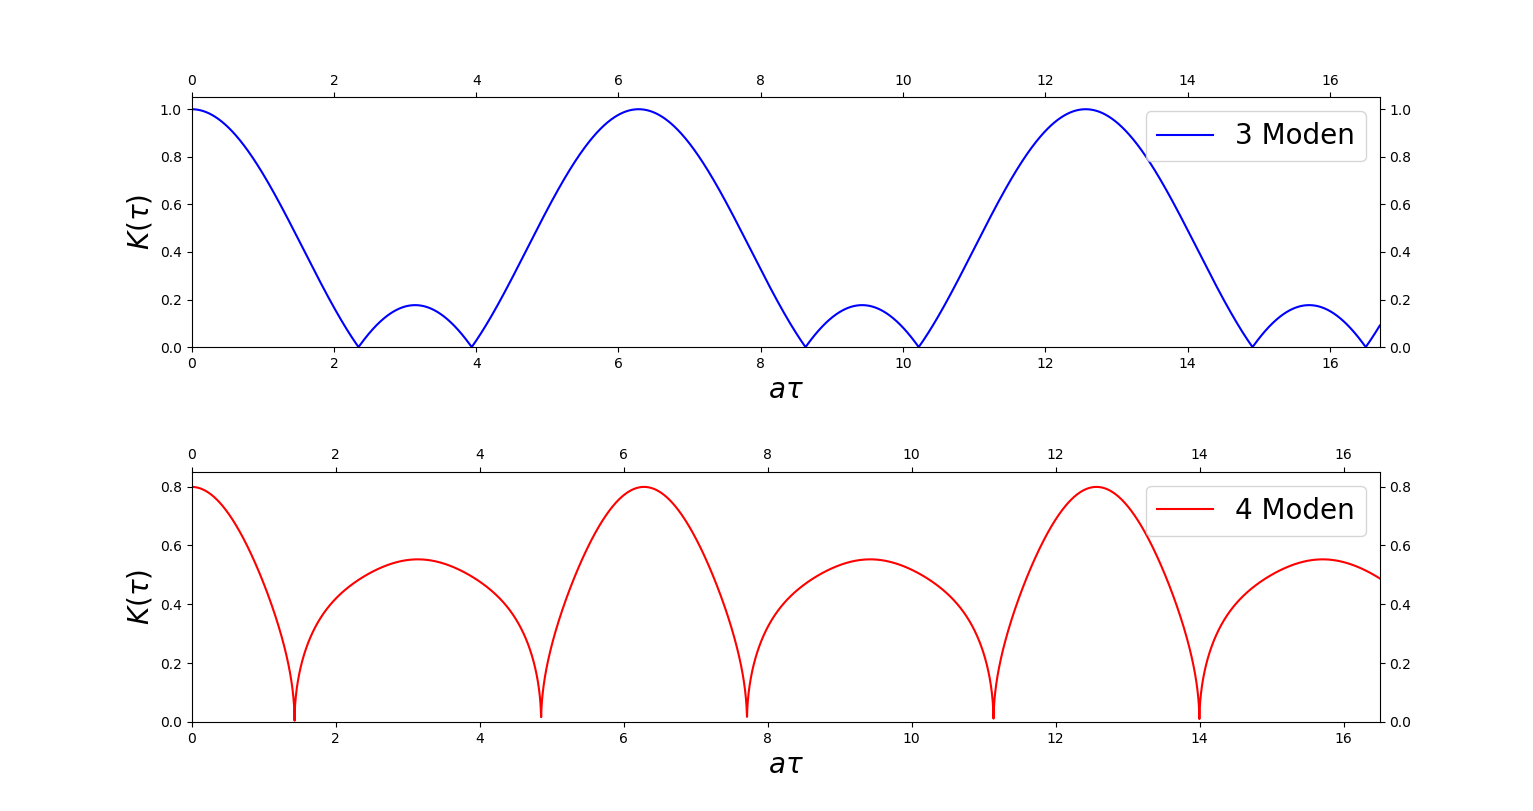
\includegraphics[scale=0.4]{Kontrast_3_und_4_Moden.png}
\caption{Der Interferenzkontrast \(K(\tau)\) für einen Helium-Neon-Laser mit drei beziehungsweise vier angeregten Lasermoden in jeweils bester Modennäherung.}
\label{Kontrast_real}
\end{figure} \\\\
Zum Vergleich geben wir entsprechende Werte für Gasentladungslampen an: 
\begin{itemize}
\item Eine Hochdruck-Gasentladungslampe mit Quecksilber als Leuchtstoff arbeitet bei Temperaturen im Bereich \(T = 3200 \hdots 4200 \ \mathrm{K}\). Von den besonders intensiven Spektrallinien liegen fünf im UV-Bereich, zwei an der blauvioletten Grenze des sichtbaren Lichts und eine Doppellinie im orangen Bereich. Nur die letzte wäre für holographische Anwendungen sinnvoll, da sie deutlich sichtbar ist. Die Wellenlänge von \(\lambda = 597 \ \mathrm{nm}\) ist im Rahmen einer Modellrechnung mit der vom Helium-Neon-Laser vergleichbar. Für diese Linie erhält man folgende Kreisfrequenz und Standartabweichung durch Dopplerverbreiterung:
\begin{align*}
\Omega = \frac{2\pi c}{\lambda} = 3.26\cdot 10^{15} \ \mathrm{Hz} \quad\quad \sigma = \sqrt{\frac{k_{\mathrm{B}} T}{mc^2}} \Omega = 4.25 \ \mathrm{GHz} \quad\text{bei} \ T = 3700 \ \mathrm{K}
\end{align*}
Unter der Annahme einer gaußförmigen Verteilung erhält man dann folgende Kohärenzlänge:
\begin{align*}
\tau_{\mathrm{C}} = \frac{\sqrt{2}}{\sigma} = 3.33\cdot 10^{-10} \ \mathrm{s} \quad\Longrightarrow\quad\underline{\underline{l_{\mathrm{C}} = 10.0 \ \mathrm{cm}}}
\end{align*}
\item Natriumdampflampen in Niedrigdruckausführung arbeiten bei einer deutlich geringerer Temperatur von etwa \(T = 600 \ \mathrm{K}\). Markant ist hier besonders die \(D\)-Linie bei \(\lambda = 589 \ \mathrm{nm}\), die sich aufgrund der ähnlichen Größenordnung ebenfalls gut für eine Modellrechnung eignet. Hier erhält man für die Kreisfrequenz:
\begin{align*}
\Omega = \frac{2\pi c}{\lambda} = 3.20\cdot 10^{15} \ \mathrm{Hz} \quad\quad \sigma = \sqrt{\frac{k_{\mathrm{B}} T}{mc^2}} \Omega = 4.97 \ \mathrm{GHz} \quad\text{bei} \ T = 600 \ \mathrm{K}
\end{align*}
und für die Kohärenzlänge:
\begin{align*}
\tau_{\mathrm{C}} = \frac{\sqrt{2}}{\sigma} = 2.85\cdot 10^{-10} \ \mathrm{s} \quad\Longrightarrow\quad\underline{\underline{l_{\mathrm{C}} = 8.5 \ \mathrm{cm}}}
\end{align*}
\end{itemize}
Beide Beispiele zeigen, dass die Kohärenzlänge von Gasentladungslampen kleiner ist als beim Laser, aber zumindest noch in einer ähnlichen Größenordnung. Der wesentliche Unterschied, der den Laser hier auszeichnet, ist vor allem die definierte Wellenlänge: Aufgrund der Dopplerverbreiterung erhält man bei den Gasentladungslampen eine Unschärfe in der Wellenlänge von ungefähr \(\Delta\lambda_{\mathrm{Hg}} = 0.44 \ \mathrm{nm}\) für Quecksilber beziehungsweise \(\Delta\lambda_{\mathrm{Na}} = 0.37 \ \mathrm{nm}\) für Natrium. Dieser Fehler von knapp \(7 \%\) sorgt dafür, dass die Spektrallinien nicht mehr scharf genug definiert sind um ein Hologramm anzufertigen. Beim Laser ist das Gaußpaket zwar ähnlich breit, aber aufgrund der filternden Wirkung des Resonators enthält das Paket kein Kontinuum an Wellenlängen sondern nur wohldefinierte Linien.

\subsection{Volumen-Phasen-Reflexions-Hologramme}
Die in diesem Versuch verwendeten Hologramme sind sogenannte Volumen-Phasen-Reflexions-Hologramme. Bei diesen wird das Interferenzmuster dreidimensional mit Hilfe einer dicken photographischen Schicht aufgezeichnet. Dies geschieht dann in Form eines Brechungsindexmusters. 
\newline
Bei der Rekonstruktion fällt dann die Referenzwelle von der Betrachterseite aus auf das Hologramm. Diese Reproduktion kann durch die Beugung der eingestrahlten Welle an einer dreidimensionalen Struktur beschrieben werden. Es muss allerdings berücksichtigt werden, dass die Referenzwelle eine Phasenverschiebung erfährt, die proportional zum lokalen Brechungsindex ist.
\section{Durchführung}
Nach einer einführenden Sicherheitsbelehrung zum Verhalten im Laser-Labor wurde zuerst das Michelson-Interferometer justiert. Dabei wird jedes Mal, wenn ein neues optisches Gerät eingebaut wurde, der Strahlengang des Lasers kontrolliert. Aufgrund der aktuellen Gegebenheiten im Labor konnte die Apparatur nicht nach den Abmessungen laut Praktikumsanleitung aufgebaut werden. In der folgenden Abbildung ist der schematische Aufbau sowie die von uns verwendeten Abmessungen dargestellt: \\\\
% Hier kommt ein Bild vom Michelson-Interferometer rein.
Nach dem Aufbau erfolgte die Feinjustage um ein möglichst deutliches und gleichmäßig ausgeleuchtets Interferenzmuster zu erhalten. Der oben dargestellte Interferometer-Arm von \(10 \ \mathrm{cm}\) Länge blieb während des gesamten ersten Teils fest justiert. Die Länge des anderen Arms wurde schrittweise erhöht und dabei das Interferenzmuster beobachtet. Der Kontrast änderte sich dabei deutlich und wurde rein visuell abgeschätzt. Dazu stand eine Übersicht zur Verfügung, in der das Interferenzbild zu verschiedenen Kontrasten vom Computer berechnet wurde. Wir haben dafür die folgenden Werte ermittelt: \\\\
\begin{table}\centering
\begin{tabular}{|c|c|c|c|c|c|c|c|c|c|}\hline
\(l / \mathrm{cm}\) & & & & & & & & &  \\\hline
\(K\) & & & & & & & & & \\\hline
\end{tabular}
\end{table}
Die Messwerte sind tatsächlich nur eine recht grobe Näherung. Als Unsicherheiten muss man etwa \(\Delta l \approx 0.1 \ \mathrm{cm}\) und \(\Delta K \approx 0.1\) annehmen. Ein genaueres Ergebnis erhält man, indem man das Interferenzmuster digital aufzeichnet und dann von einem geeigneten Programm die hellen und dunklen Pixel zählen lässt. Daraus ergäben sich dann minimale und maximale Intensitäten und somit der Kontrast. \\\\
Ziel dieses ersten Teilversuches war die Bestimmung der Modenzahl des Lasers sowie der Kohärenzlänge - ein entscheidender Schritt für ein gutes Hologramm. Da das Laserspektrum - wie die Vorbetrachtung gezeigt hat - sehr sensitiv von der Anzahl der Lasermoden abhängt, genügt die einfache qualitative Untersuchung des Verlaufes der Kontrastfunktion um die Modenzahl zu bestimmen.
    % Bibliographie/Literaturverzeichnis
    \begin{thebibliography}{9}
    \bibitem{wiki:Intensität}
    Wikipedia,
    \emph{Intensität (Physik)},
    \url{https://de.wikipedia.org/wiki/Intensit%C3%A4t_(Physik)},
    25.\,Okt.~2019.
    \end{thebibliography}

% Ende Dokument
\end{document}
